%%%%%%%%%%%%%%%%%%%%%%%%%%%%%%%%%%%%%%%%%
% Frequently Asked Questions
% LaTeX Template
% Version 1.0 (22/7/13)
%
% This template has been downloaded from:
% http://www.LaTeXTemplates.com
%
% Original author:
% Adam Glesser (adamglesser@gmail.com)
%
% License:
% CC BY-NC-SA 3.0 (http://creativecommons.org/licenses/by-nc-sa/3.0/)
%
%%%%%%%%%%%%%%%%%%%%%%%%%%%%%%%%%%%%%%%%%

\documentclass[11pt]{article}

\usepackage[margin=1in]{geometry} % Required to make the margins smaller to fit more content on each page
\usepackage[linkcolor=blue]{hyperref} % Required to create hyperlinks to questions from elsewhere in the document
\hypersetup{pdfborder={0 0 0}, colorlinks=true, urlcolor=blue} % Specify a color for hyperlinks
\usepackage{todonotes} % Required for the boxes that questions appear in
\usepackage{tocloft} % Required to give customize the table of contents to display questions
\usepackage{microtype} % Slightly tweak font spacing for aesthetics
\usepackage{palatino} % Use the Palatino font

\usepackage[utf8x]{inputenc}
\usepackage{sidecap}

\setlength\parindent{0pt} % Removes all indentation from paragraphs

% Create and define the list of questions
\newlistof{questions}{faq}{\large Sections} % This creates a new table of contents-like environment that will output a file with extension .faq
\setlength\cftbeforefaqtitleskip{4em} % Adjusts the vertical space between the title and subtitle
\setlength\cftafterfaqtitleskip{1em} % Adjusts the vertical space between the subtitle and the first question
\setlength\cftparskip{.3em} % Adjusts the vertical space between questions in the list of questions

% Create the command used for questions
\newcommand{\question}[1] % This is what you will use to create a new question
{
\refstepcounter{questions} % Increases the questions counter, this can be referenced anywhere with \thequestions
%\par\noindent % Creates a new unindented paragraph
\phantomsection % Needed for hyperref compatibility with the \addcontensline command
\addcontentsline{faq}{questions}{#1} % Adds the question to the list of questions
\todo[inline, color=green!40]{\textbf{#1}} % Uses the todonotes package to create a fancy box to put the question
\vspace{1em} % White space after the question before the start of the answer
}

% Uncomment the line below to get rid of the trailing dots in the table of contents
\renewcommand{\cftdot}{}

% Uncomment the two lines below to get rid of the numbers in the table of contents
%\let\Contentsline\contentsline
%\renewcommand\contentsline[3]{\Contentsline{#1}{#2}{}}


\ifdefined\frenchmanual
  \newcommand\mtext[2]{#1}
\else
  \newcommand\mtext[2]{#2}
\fi



\begin{document}

%----------------------------------------------------------------------------------------
%	TITLE
%----------------------------------------------------------------------------------------


\begin{flushright}
  
\includegraphics[width=0.1\textwidth]{bretagne_quadri.pdf}
\end{flushright}

\begin{center}
\Huge{\bf \emph{\mtext{Wi2Me User - Manuel d'utilisation}{Wi2Me User - User Manual}}} % Main title
\end{center}

\begin{flushleft}
\todo[inline, color=green!40]{\textbf{\mtext{Introduction et Contact}{Introduction and Contact}}} % Uses the todonotes package to create a fancy box to put the question
\mtext{Ce document présente l'utilisation de l'application de mesure Wi2Me User développée par TELECOM Bretagne. Pour plus d'information ou de support :}{This Document presents the steps required to perform mesurements using the Wi2Me User application developed by TELECOM Bretagne.}

%\mtext{}{ For more information or support, feel free to contact : }
%Tanguy Kerdoncuff \\ 
%tanguy.kerdoncuff@telecom-bretagne.eu\\
%+332 99 12 70 49 \\
%TELECOM Bretagne - Dept. RSM\\
%2, Rue de la Chataigneraie \\
%35100 Cesson Sévigné\\
\end{flushleft}

\listofquestions % This prints the subtitle and a list of all of your questions

\newpage % Comment this if you would like your questions and answers to start immediately after table of questions
%----------------------------------------------------------------------------------------
\question{\mtext{Générer une Trace}{Generating a Trace}}\label{starting}
\textbf{IMPORTANT : }
  \mtext{NOTIMPL}{ The wi2me application generated databases of wireless information called "Traces". As many traces can afterwards be combined by our processing tool, it is more efficient to make a new database for each different mesurements. The generation of a new Trace is made during the "Extracting the mesurements" phase described further in this document. This lets you start and stop the application if you need to make a pause during mesurements, or if you run out of battery. On another hand, do not forget to extract the data between two unrelated mesurement sessions.}

%----------------------------------------------------------------------------------------
\question{\mtext{Lancer Wi2Me}{Starting Wi2Me}}\label{starting}

 
\mtext{NOTIMPL}{Once the application is up and ruinning, it is easy to start the application using the START button.}
\centering
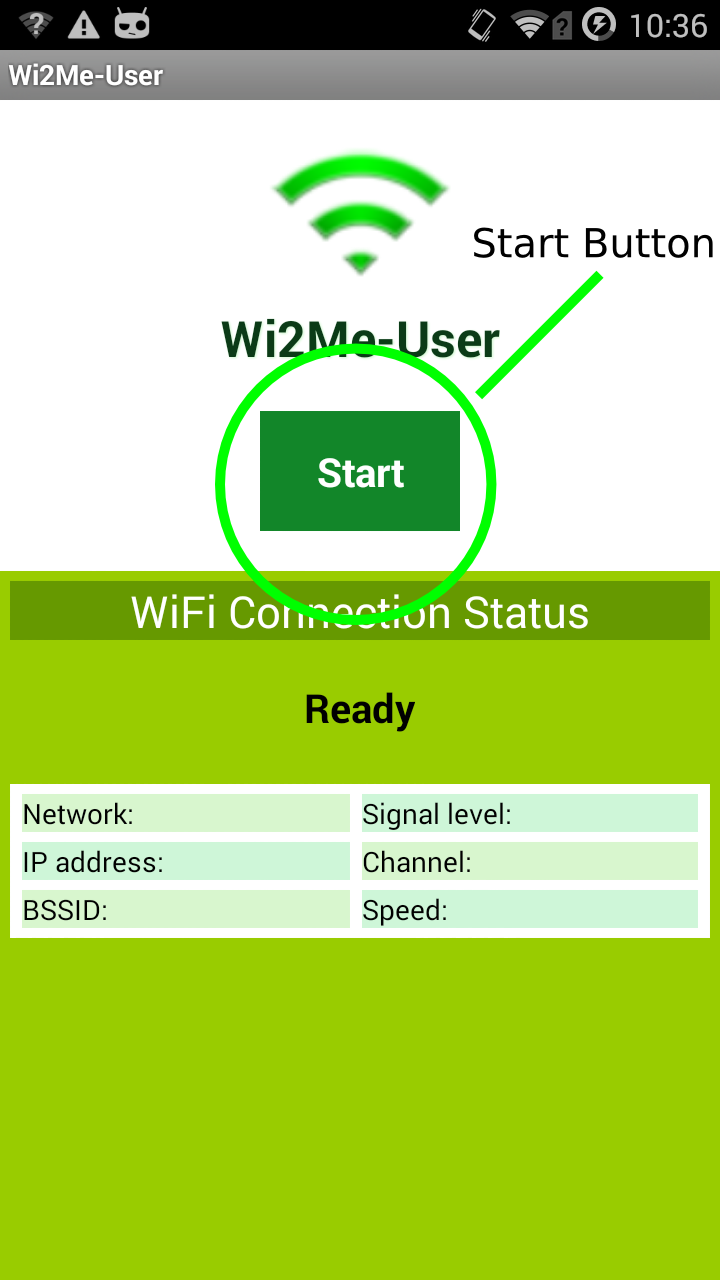
\includegraphics[height=0.35\textheight]{figures/start_screen.png}
\flushleft

%------------------------------------------------
\question{\mtext{Arrêter wi2me}{Stopping Wi2Me}}\label{stopping}
  \mtext{NOTIMPL}{Stopping the mesurements is done in a similar fashion using the STOP button.}\\
\centering
  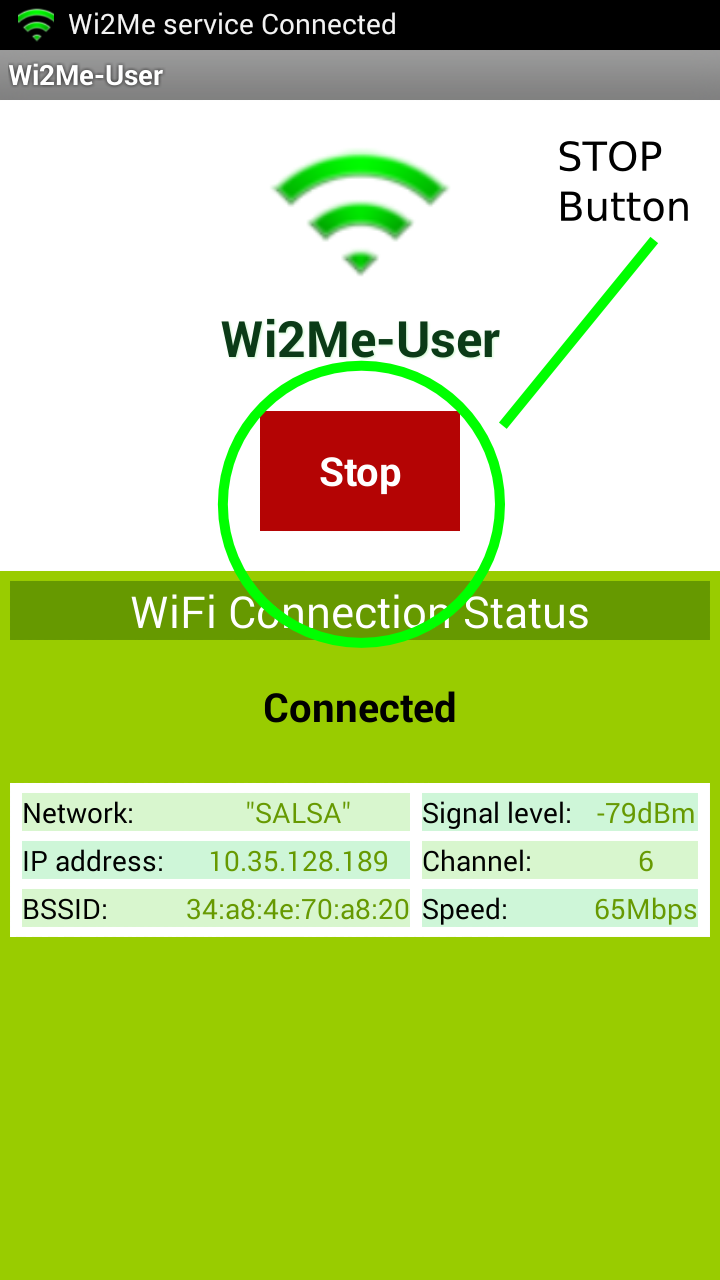
\includegraphics[height=0.35\textheight]{figures/stop_screen.png}
\flushleft

\question{\mtext{Extraire les mesures}{Extracting the mesurements}}\label{upload}
  \mtext{NOTIMPL}{Retrieving the mesurement is done from the application's menu (summoned using the phone's physical or onscreen menu touch). The Upload button will then send the traces to the wi2me server, but a copy is kept locally in \emph{/sdcard/Wi2MeUser/traces/} . \textbf{NOTE : Even if the phone has no connectivity, the upload button will keep a local copy in the aforementionned folder.} In many cases, this should be enough.}\\
\centering
  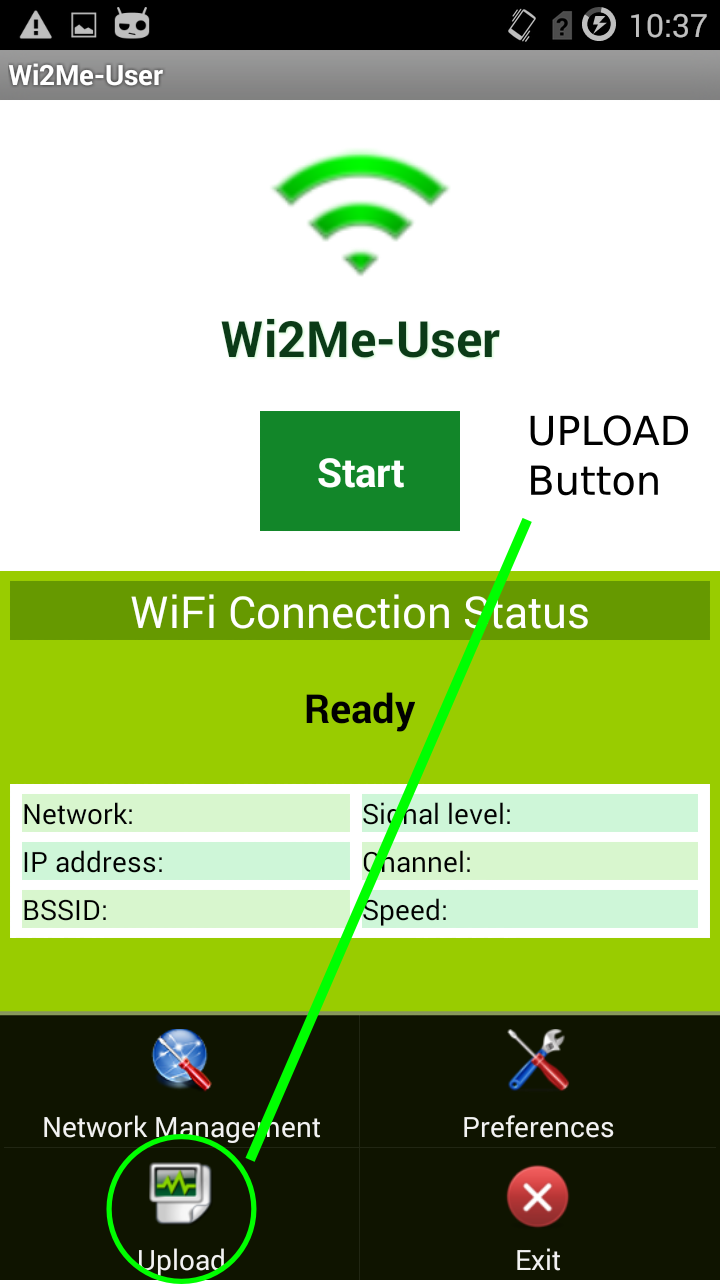
\includegraphics[height=0.35\textheight]{figures/upload_screen.png}
\flushleft

\end{document}
